\chapter{Sistemas de Información Geográfica}
\label{ch:geopackage}

\begin{chapsummary}
	Partimos con la explicación de qué es y de qué se compone la información geográfica, así como explicando los dos principales modelos de representación. Después, detallamos cómo se almacena esta y aquellos contenedores de datos más comunes.
\end{chapsummary}

\section*{Introducción} En este capítulo, se pretende dar a conocer sobre los \textit{GIS}, \textit{Sistemas de la Información Geográfica} (del inglés \textit{Geographical Information Systems}), formado por aquellas herramientas que trabajan con información geográfica, sea manipulación, almacenamiento o visualización.

\section{Información Geográfica}
	La información geográfica es aquella que está georreferenciada, es decir, que tiene alguna referencia geográfica asociada. Es inmediato la posible división de esta en dos, las componentes espacial y temática \autocite[69]{volaya}.
	
	La componente temática corresponde a todo dato no espacial que contextualice, aporte más información sobre qué representa esa marca geográfica, mientras que la componente espacial tiene una estructura a modelos en tres niveles\autocite[80]{volaya}:
	
	\begin{description}
		\item[\textbf{Modelo Geográfico}] Modelo conceptual de la realidad geográfica y el comportamiento de esta.
		\item[\textbf{Modelo de Representación}] Conjunto finito de elementos que representa las características del modelo anterior.
		\item[\textbf{Modelo de Almacenamiento}] Esquema de cómo almacenar los distintos elementos usados para la representación.
	\end{description}
	
\subsection{Modelo Ráster}
	Es un modelo en el que los datos están ordenados en cuadrillas o celdas uniformemente espaciadas. En cada celda se encuentra un valor, que representa algo, generalmente una clasificación o un valor dentro de un espectro. 
	
	\begin{figure}[htbp]
		\centering
		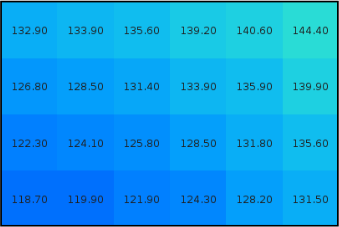
\includegraphics[width=0.65\textwidth]{models_raster}		
		\caption[Representación de datos geográficos de tipo ráster]{La información tipo ráster suele ser representada como una matriz numérica o alfanumérica. {Fuente: \autocite[86]{volaya}}}
	\end{figure}
	
	Esta propiedad de separación uniforme es muy interesante pues, aún siendo rígida como composición, se puede usar para afinar la granularidad de los datos, el ámbito de estos.
	
	Posibles usos para estos puede incluir clasificación o Modelos Digitales del Terreno que definan elevación, sentido de bajada de flujos como la lluvia, entre otros.

\subsection{Modelo Vectorial}
	El modelo vectorial es aquel en el que la información se representa con formas geométricas. Esto, en contraposición al modelo anterior, nos permite mayor flexibilidad a la hora de dar representación. Esto, por ejemplo, nos permite asignar clasificaciones a zonas de diferente tamaño y forma.
	
	Existen tres primitivas de tipo vectorial \autocite[92-95]{volaya}: puntos, líneas y polígonos.

\begin{description}
	\item[\textbf{Puntos}] Elementos compuestos por coordenadas espaciales.
	\item[\textbf{Líneas}] Sucesión ordenada de puntos. Pueden ser cerradas o abiertas, dependiendo de si coincide o no el primer y último punto.
	\item[\textbf{Polígonos}] Línea cerrada que delimita un área. Puede tener o no líneas interiores que delimiten un hueco vacío.
\end{description}

Estos elementos pueden almacenarse formas textuales o binarias, respectivamente, en \textit{WKT} (\textsc{Well-Known Text}) o \textit{WKB} (\textsc{Well-Known Binary}).

\begin{figure}[htbp]
	\begin{subfigure}{0.32\textwidth}
		\centering
		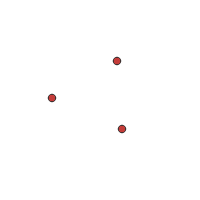
\includegraphics[width=.95\textwidth]{img/models_vector_points.png}
		\subcaption{Puntos}
	\end{subfigure}
	\begin{subfigure}{0.32\textwidth}
		\centering
		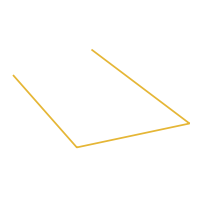
\includegraphics[width=.95\textwidth]{img/models_vector_lines.png}
		\subcaption{Líneas}
	\end{subfigure}
	\begin{subfigure}{0.32\textwidth}
		\centering
		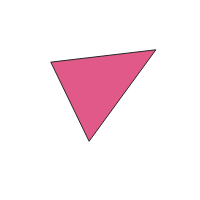
\includegraphics[width=.95\textwidth]{img/models_vector_poly.png}
		\subcaption{Polígonos}
	\end{subfigure}
	\caption[Tipos básicos de los elementos vectoriales]{Elementos vectoriales primitivos, los bloques de construcción básicos que definen la información geográfica vectorial.}
\end{figure}

\section{Contenedores de Datos}
	Se acostumbra a almacenar la información geográfica en bases de datos \autocite[203-227]{volaya} bien definidas, minimizando los recursos necesarios para su almacenamiento y facilitando su uso y transmisión, así como liberando de posibles dependencias a aplicaciones concretas.

	Dentro del sector, existen varios estándares, entre ellas bases de datos planas como \textit{Shapefile} de \textit{ESRI}, \texttt{GeoJSON}\footnote{\texttt{GeoJSON}: Extensión geográfica del formato de serialización \texttt{JSON}. \url{https://geojson.org/}} e incluso \texttt{CSV}\footnote{\texttt{CSV}: Valores separados por coma, formato muy sencillo y de temática agnóstica.}. Por otra parte, existen bases de datos relacionales, como \textit{Microsoft SQL Server} o \textit{PostgreSQL} con su extensión \textit{PostGIS}. En un punto intermedio, podemos encontrar el llamativo y novedoso \textit{GeoPackage}, sujeto de estudio en este trabajo.

\subsection{\textit{ESRI Shapefile}}
	\textit{Shapefile}, desarrollado por \textit{ESRI}\footnote{ESRI: Empresa dominante en la industria, con grandes aportes e influencia, así como desarrolladores de \textit{ArcGIS}. \url{https://www.esri.com/}}, es un formato vectorial en el que los datos se dividen en varios archivos.
	
	Aunque su uso es muy extenso incluso llegándose a considerarse \textit{lingua franca} del mundo \textit{GIS}, este formato es, en realidad, una reliquia del pasado. Desarrollado para un uso interno del software \textit{ArcView} de \textit{ESRI}, el formato era muy útil y novedoso, y gran cantidad de información fue codificada en este al liberarse la descripción técnica\footnote{Descripción técnica de Shapefile. \url{https://www.esri.com/library/whitepapers/pdfs/shapefile.pdf}} para que otros GIS pudiesen usarlos.
	
	Dado su origen, en propósito y época, el formato tiene muchas limitaciones como:
	
	\begin{itemize}
		\item Existe un máximo de almacenamiento, 2GB de espacio, así que no es utilizable en casos de grandes colecciones de información.
		\item El nombre de los atributos, de las columnas está restringido a 10 caracteres de máximo.
		\item Es un formato \textit{ASCII} y no acepta \textit{Unicode} para codificar idiomas que no compartan el alfabeto inglés.
		\item Existe un máximo de 255 atributos.
		\item Los números decimales son almacenados como texto, y por tanto pueden contener errores de redondeo.
	\end{itemize}

	En esencia, \textit{Shapefile} es una base de datos plana muy capaz, pero con severas limitaciones que causan molestia o imposibilitan ciertas tareas.

\subsection{\textit{PostgreSQL} y \textit{PostGIS}}
	\textit{PostgreSQL} es una base de datos relacional muy extensible y con gran cantidad de características, aunque no goza de soporte \textit{GIS} de base. Para eso, está la extensión \textit{PostGIS}, que dota a una base de datos \textit{PostgreSQL} con soporte para interpretar datos vectoriales, textuales o binarios, así de múltiples funciones \textit{SQL} para trabajar con datos geográficos en consultas u operaciones \autocite[6-10]{obehsu}.
	
	En definitiva, \textit{PostGIS} (como extensión de \textit{PostgreSQL}) es un software muy capaz, proporcionando una base de datos relacional con características \textit{GIS} pero que no tiene cabida en ciertos entornos más limitados en recursos, como terminales móviles. Otra base de datos reseñable que compite con \textit{PostGIS} es \textit{SQL Server} de \textit{Microsoft}, aunque también comparte las mismas pegas.

\subsection{\textit{GeoPackage}}
	\textit{GeoPackage}, como estándar de la \textit{OGC}, se halla en un punto intermedio entre ambos, digamos una adaptación moderna de \textit{Shapefile} puesto que es una base de datos contenida en un único fichero con similitud a \textit{PostgreSQL} ya que dicho fichero es en realidad una base de datos relacional \textit{SQLite}\footnote{\textit{SQLite}: Base de datos relacional de dominio público cuya principal virtud es su existencia en un único archivo. \url{https://www.sqlite.org}}.
	
	Al contenerse en un solo archivo, su almacenamiento y copia es sumamente sencillo, simplificando el envío masivo de información por, por ejemplo, correo electrónico. En contraposición, al ser un archivo binario, es complicado su serialización y transmisión por la red, ya que no hay puntos bien delimitados donde empiece y acabe la estructura.
	
	Al tratarse de una base de datos relacional, esto le permite relacionar diferentes entidades relacionadas entre sí, como por ejemplo datos de las calles de un municipio y la descomposición topológica de dichas calles. Por desgracia, como es un simple contenedor, a diferencia de herramientas como \textit{Spatialite}\footnote{\textit{Spatialite}: Herramienta para dotar de capacidades \textit{GIS} a una base de datos \textit{SQLite}. \url{https://www.gaia-gis.it/fossil/libspatialite/index}} o \textit{PostGIS}, no dispone de tantas funciones para operar con primitivas, y tiene una fuerte dependencia en las herramientas.
	
	En esencia, la mayor limitación que tiene \textit{GeoPackage} es simplemente su corta edad. Esto es así porque, frente a otros competidores, no existen tantas herramientas que trabajen con \textit{GeoPackage} como formato. La solución para esto es simple y orgánica, ya que con el tiempo se desarrollan nuevas herramientas y maduran las ya existentes.
	
	 